\section{Auswertung}
    \subsection{Kenngrößen des Beheizbaren Ringkern}
        Zunächst wurde für die Beheizbare Spule mit Ringkern bei Raumtemperatur für verschiedenen Stromstärken je eine Hysteresenkurve aufgenommen um daraus anschließend die Remanenz-, Koerzitivfeldstärke und Maximale Magnetisierung
        zu bestimmen.
        Dafür konnten die Kenngrößen aus folgenden Graphen abgelesen Werden
        \begin{figure}[ht]
            \centering
            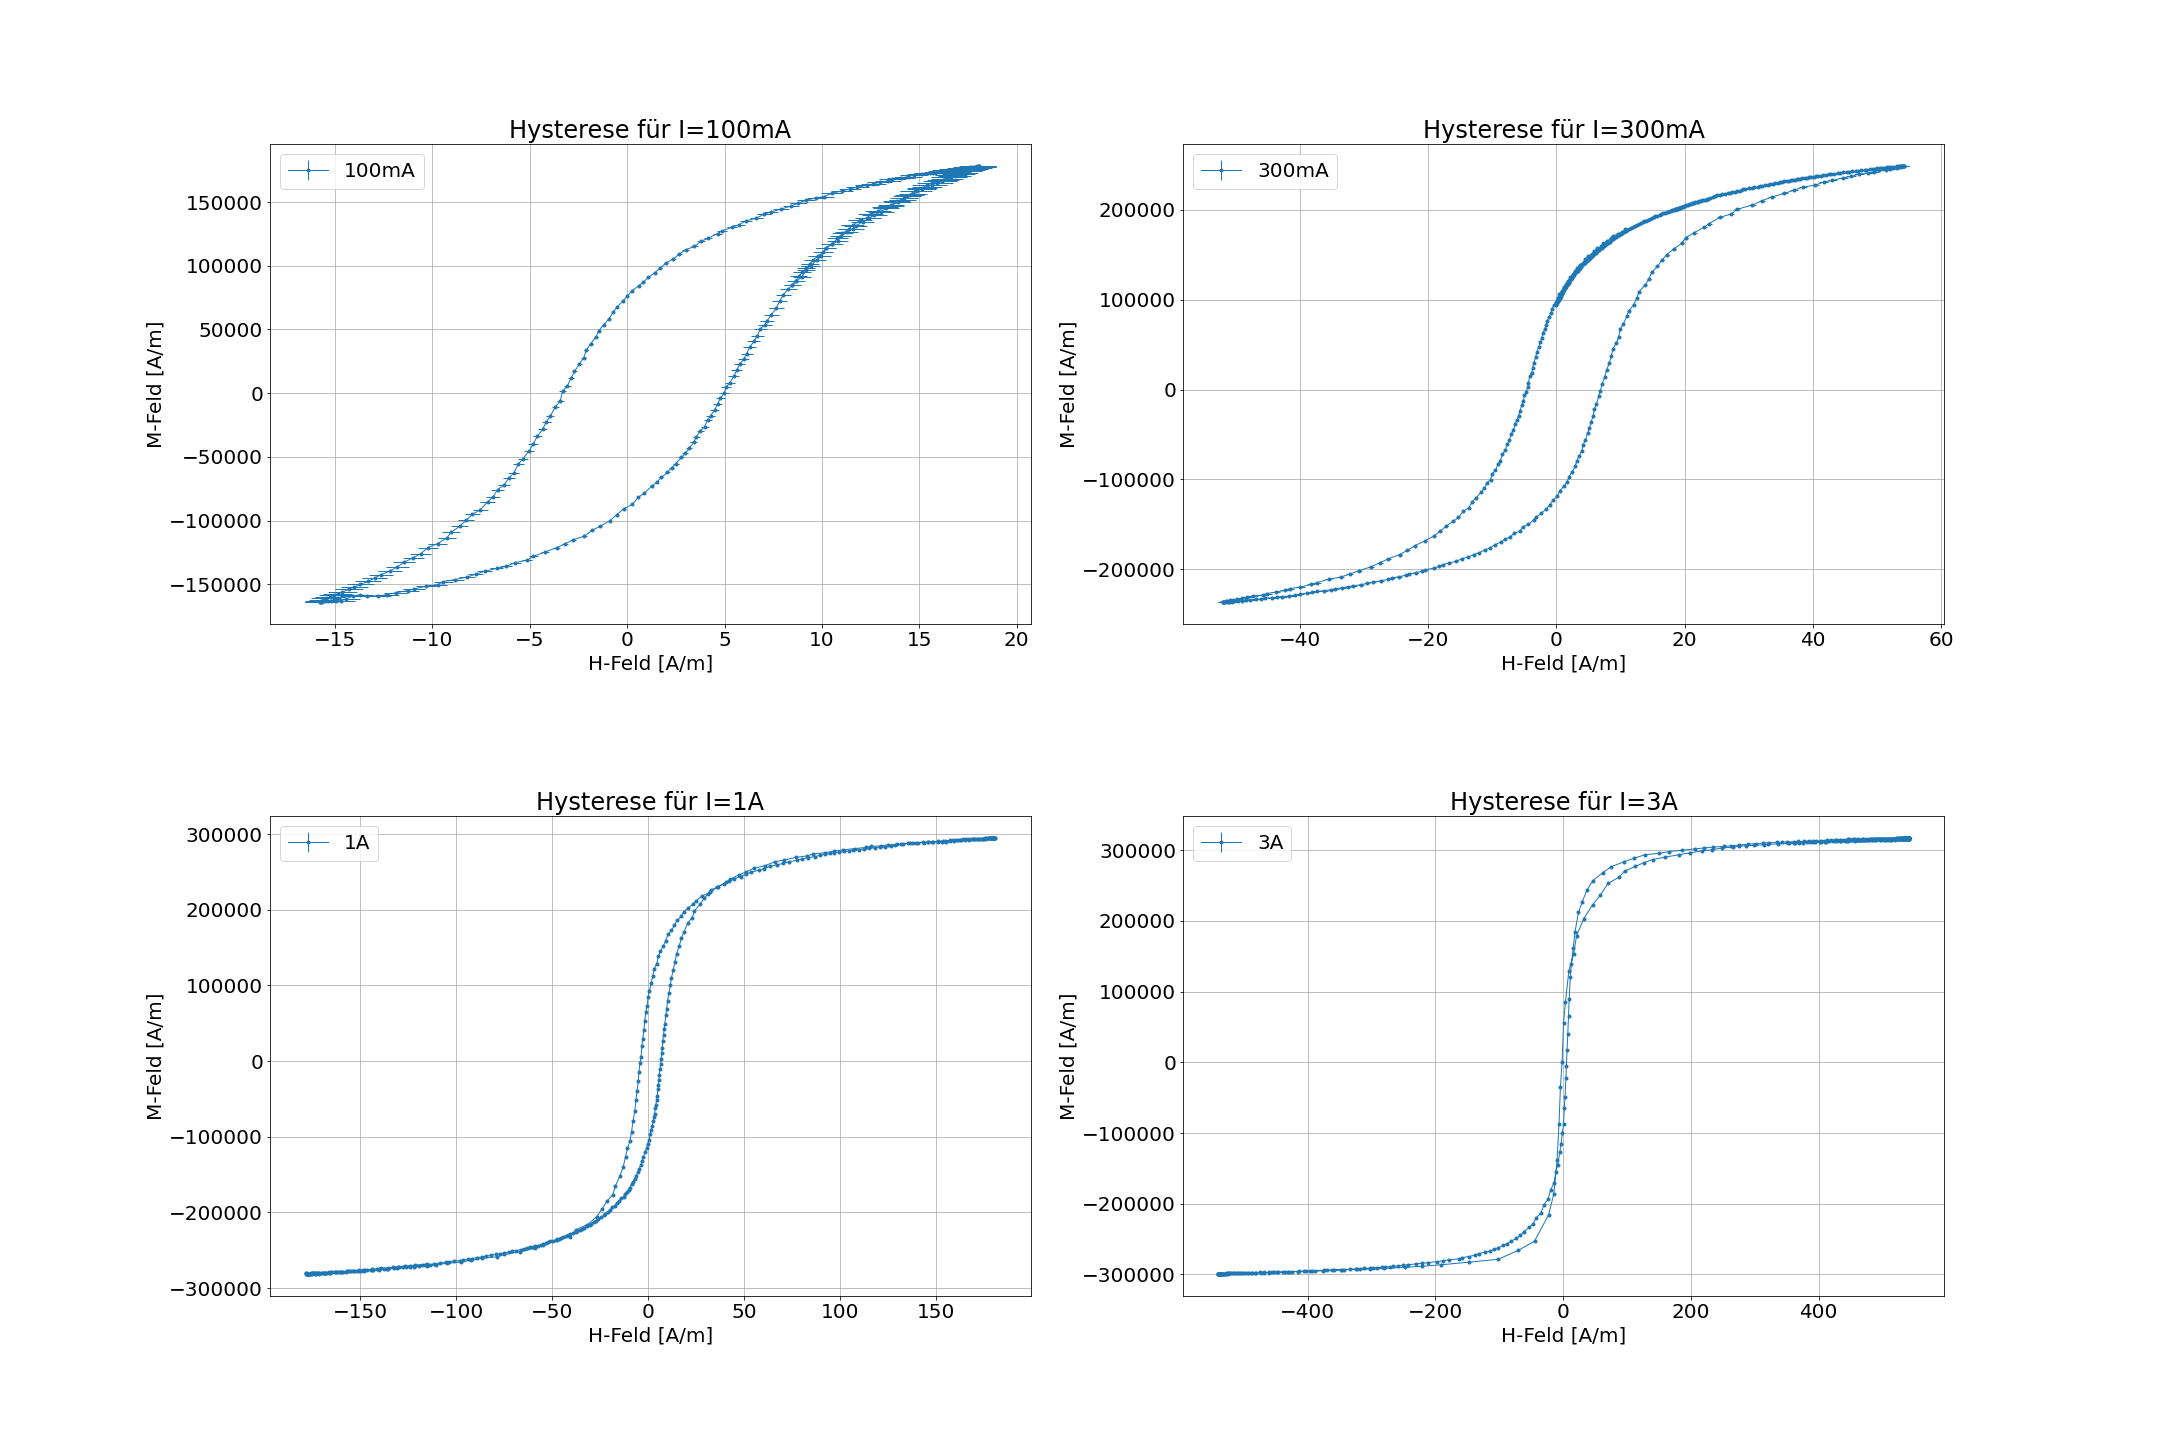
\includegraphics[width=\textwidth]{Images/Teil1.PNG}
            \label{Hysteresen}
            \caption{Hysteresenkurven bei Stromstärken 100mA,300mA,1A und 3A}
        \end{figure}
        Daraus lies sich folgende Tabelle zusammenstellen
        \begin{table}[ht]
            \centering
            \begin{tabular}[]{c|c|c|c}
                Stromstärke & Remanenzfeldstärke [A/m] & Koerzitivfeldstärke [A/m] & Maximale Magnetisierung [A/m] \\
                \hline
                100mA & 8.36e4 & 8.3 & 17.12e4 \\
                300mA & 10.66e4 & 11.33 & 24.26e4 \\
                1A    & 9.5e4 & 10.99 & 28.84e4 \\
                3A    & 7.15e4 & 6.86 & 30.86e4 \\
            \end{tabular}
        \end{table}
        \colorbox{green}{TODO (für erik), erwartungswerte ausrechenen für Ringkernspule bei stromstärken}
        \colorbox{green}{hier theorie einfügen}, jedoch ist der Trend von streigenden maximalen Magnetisierungen entsprechend unserer Erwartungen. Die Fluktuation von sowohl Remanenzfeldstärke als auch Koerzitivfeldstärke
        wirkt hier jedoch fehl am platz, da diese nicht von der Stromstärke abhängt.
    \subsection{Kommutierungskurve und Suszeptibilität}
        Um die Suszeptibilität des Systems zu bestimmen wurde durch die Variation des Primärspulenstroms jeweils eine Kommutierungskurve für 1 bis 0 A und 3 bis 0 A aufgenommen.
        Durch fitten des modells 
        \begin{equation}
            M(H) = A \cdot exp(-\frac{b}{H} + c) + d
        \end{equation}
        wurden zwei differenzierbare Äquivalente der aufgenommen Messdaten erzeugt um anschließend die Suszeptibilität in Abhängigkeit des angelegten Magnetfeldes zu plotten.
        \begin{figure}
            \centering
            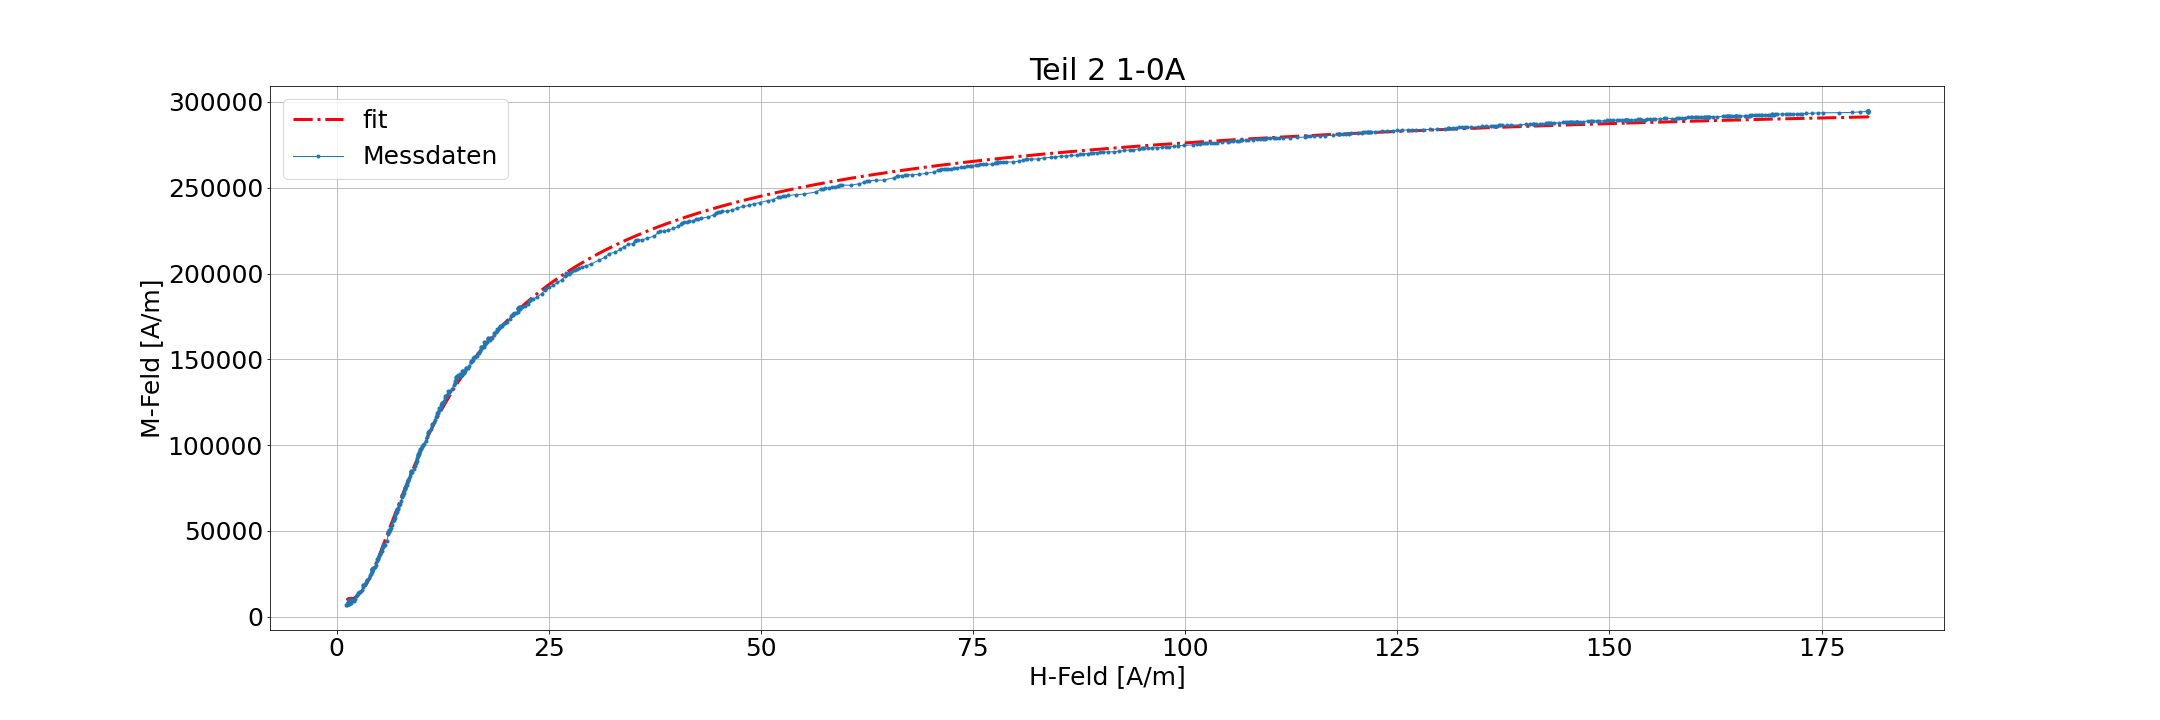
\includegraphics[width=\textwidth]{Images/Teil2Teil 2 1-0A.png}
            \label{Teil2-1A}
            \caption{Fit der Kommutierungskurve für 1 bis 0A}
        \end{figure}
        \begin{figure}
            \centering
            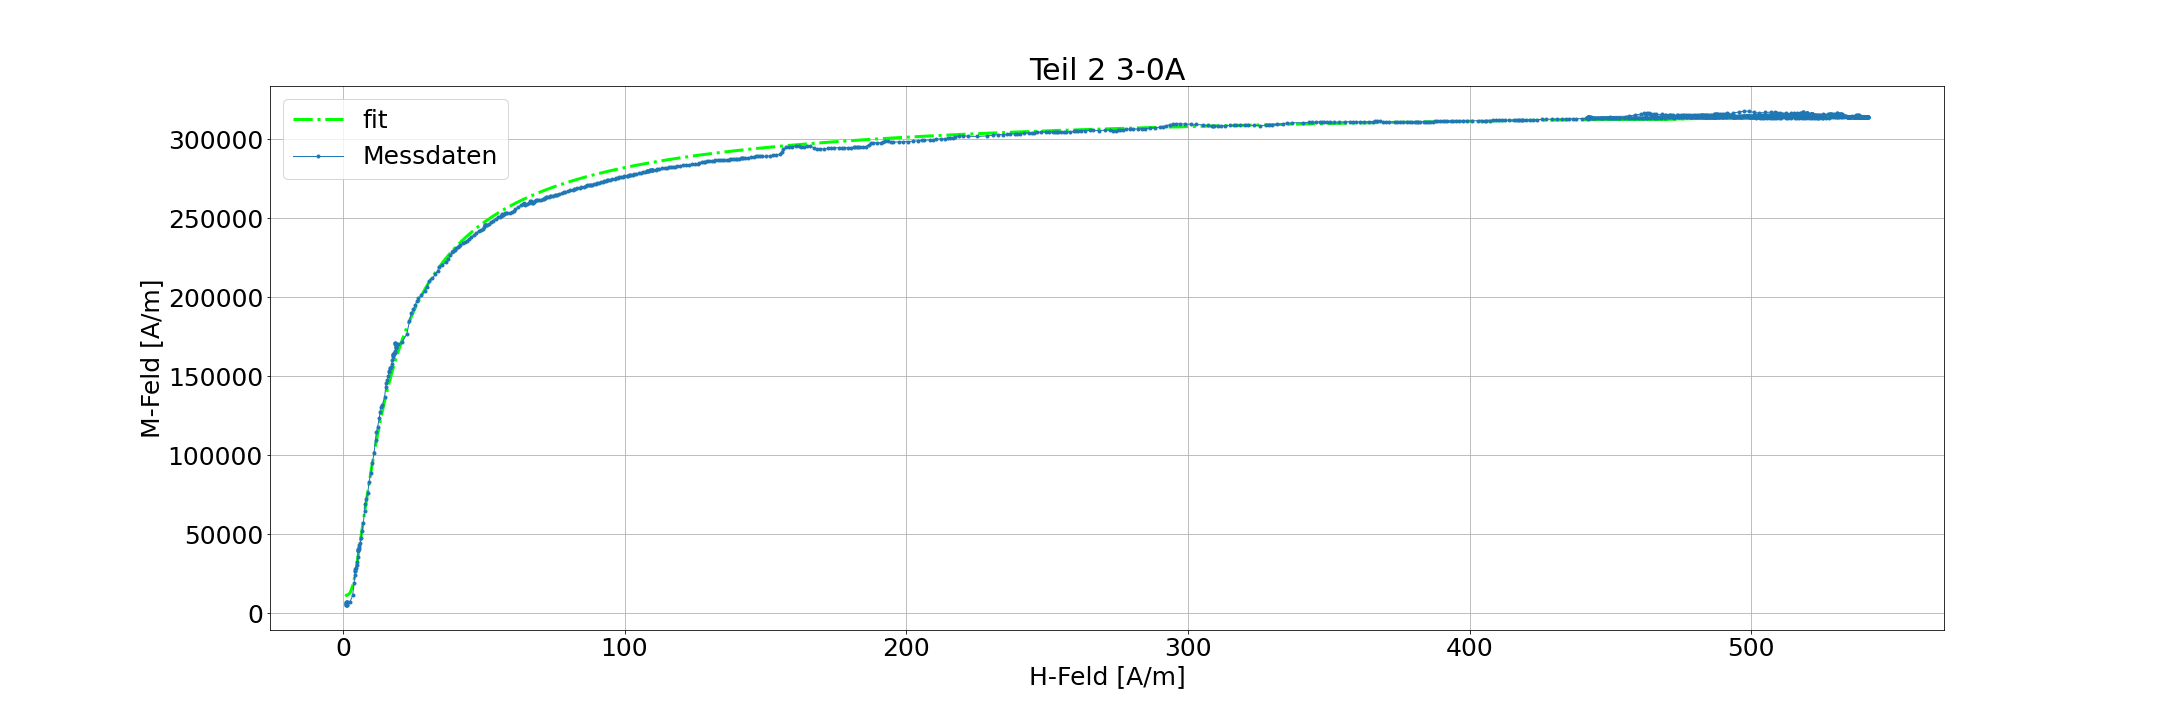
\includegraphics[width=\textwidth]{Images/Teil2Teil 2 3-0A.png}
            \label{Teil2-3A}
            \caption{Fit der Kommutierungskurve für 3 bis 0A}
        \end{figure}
        \begin{figure}
            \centering
            \includegraphics[width=\textwidth]{Images/Teil2Differentielle Suszeptibilität.png}
            \label{DiffSus}
            \caption{Plot der Suszeptibilitäten für beide Kommutierungskurven}
        \end{figure}
        \colorbox{green}{Todo (für erik) beschreibe den Verlauf}